\documentclass[12pt]{article}
\usepackage{amsmath,amssymb,amsthm}
\usepackage{graphicx}
\usepackage{float}
\usepackage{geometry}
\geometry{top=1in, bottom=1.25in, left=1in, right=1in}
\usepackage{caption}
\usepackage{subcaption}
\usepackage{pdfpages}
\usepackage{hyperref}
\hypersetup{
    colorlinks=true, 
    linkcolor=black, 
    urlcolor=blue,
    pdftitle={Project 1: Heating and Cooling of Buildings},
    pdfauthor={William Roberts, Ryan Jenkins, Evan Miller}
}
\usepackage{booktabs}
\usepackage{array}
\usepackage{mathtools}
\usepackage{bm}
\usepackage{siunitx}
\usepackage{enumitem}
\usepackage{listings}
\usepackage{xcolor}

\lstset{
  language=Matlab,
  basicstyle=\ttfamily\small,
  keywordstyle=\color{blue},
  commentstyle=\color{green!50!black},
  stringstyle=\color{orange},
  breaklines=true,
  breakatwhitespace=true,
  showstringspaces=false,
  frame=single,
  captionpos=b,
  numbers=left,           
  numberstyle=\small\color{black},  
  stepnumber=1,        
  numbersep=10pt 
}


\setlist{nosep}

\title{Project 1: Heating and Cooling of Buildings}
\author{William Roberts \and Ryan Jenkins \and Evan Miller}
\date{\today}

\begin{document}
\maketitle

\tableofcontents
\clearpage

\section{Introduction}
Billy Bob works in a specialized laboratory dedicated to studying microbial cells, where maintaining precise temperature conditions is crucial. Each day, he monitors the building’s heating and cooling systems to ensure that the microbes are kept within safe temperature ranges. Even small fluctuations in temperature could compromise experiments or damage sensitive equipment. To better understand how the indoor environment responds to various influences, Billy Bob decides to investigate the factors that control the lab's temperature. He considers the impact of the outside weather, the heat generated by internal sources, and the role of the thermostat in maintaining a stable environment for the laboratory. By combining analytical modeling with numerical simulations, he aims to predict temperature changes, identify potential risks, and develop strategies to keep the lab conditions safe and consistent.

\section{Background}
For the purposes of modeling the temperature of the building, $T$, at time $t$. The three elements Billy Bob is looking at are: the effect of the ambient outside temperature, $A(t)$, the heat produced by machinery, lights, and people, $H(t)$, and artificial heating and cooling, $Q(t)$, yielding the differential equation $ \frac{dT}{dt} = A(t) + H(t) + Q(t)$.

\section{Analytical investigation (Task Set A)}

\section{Numerical methods and verification (Task Set B)}

When using simplified versions of the temperature model, as was the case in the previous section, where $H(t)$ and $A(t)$ are assumed to be zero and $M(t)$ is assumed constant, the differential equation modeling the internal building temperature can be solved by hand. However, as the model improves, considering the effects of more of these variances, it will become impractical to perform these calculations manually. As such, it is pertinent to develop and verify a program to numerically approximate solutions to these models, in this case, the fourth-order Runge-Kutta program featured in Appendix A.

In order to test our program and verify its accuracy, we can plug in equation (?) and compare the results to the exact solution obtained in the previous section. Plotting the solutions against each other in Figure 1, we can compare the two solutions.

\begin{figure}[H]
     \centering
    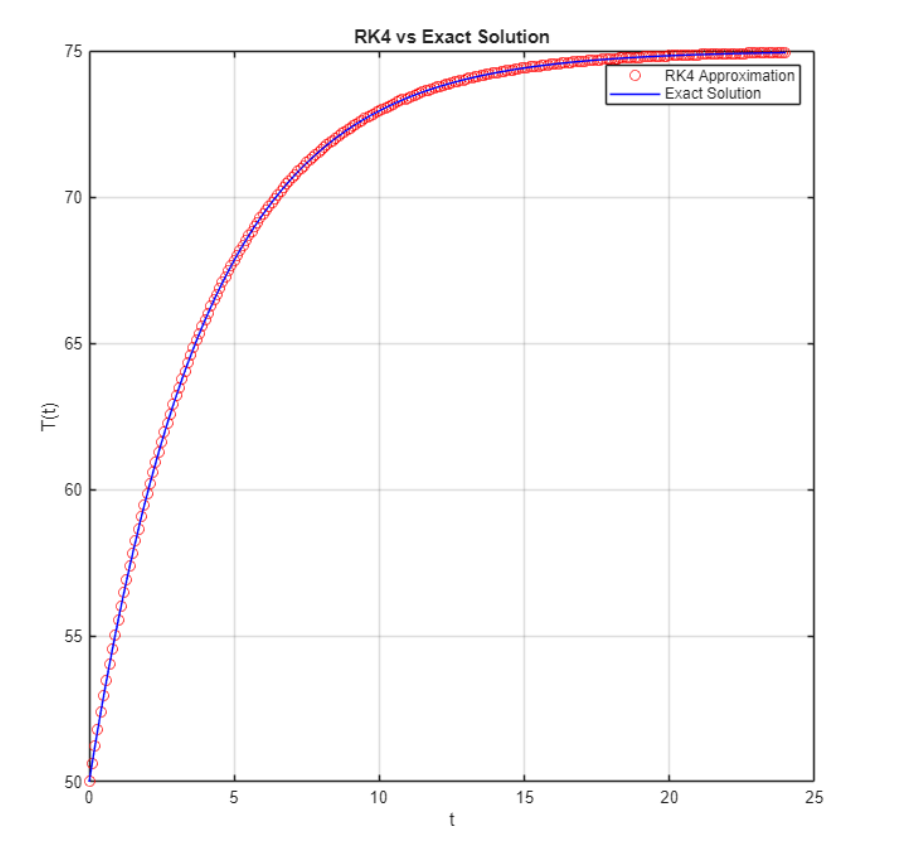
\includegraphics[width=0.5\linewidth]{Screenshot 2025-09-29 180223.png}
    \caption{Runge-Kutta fourth-order approximation vs exact solution}
    \label{fig:placeholder}
\end{figure}
   

To quantify this comparison, refer to Figure 2, plotting the error in our approximation. 

\begin{figure}[H]
    \centering
    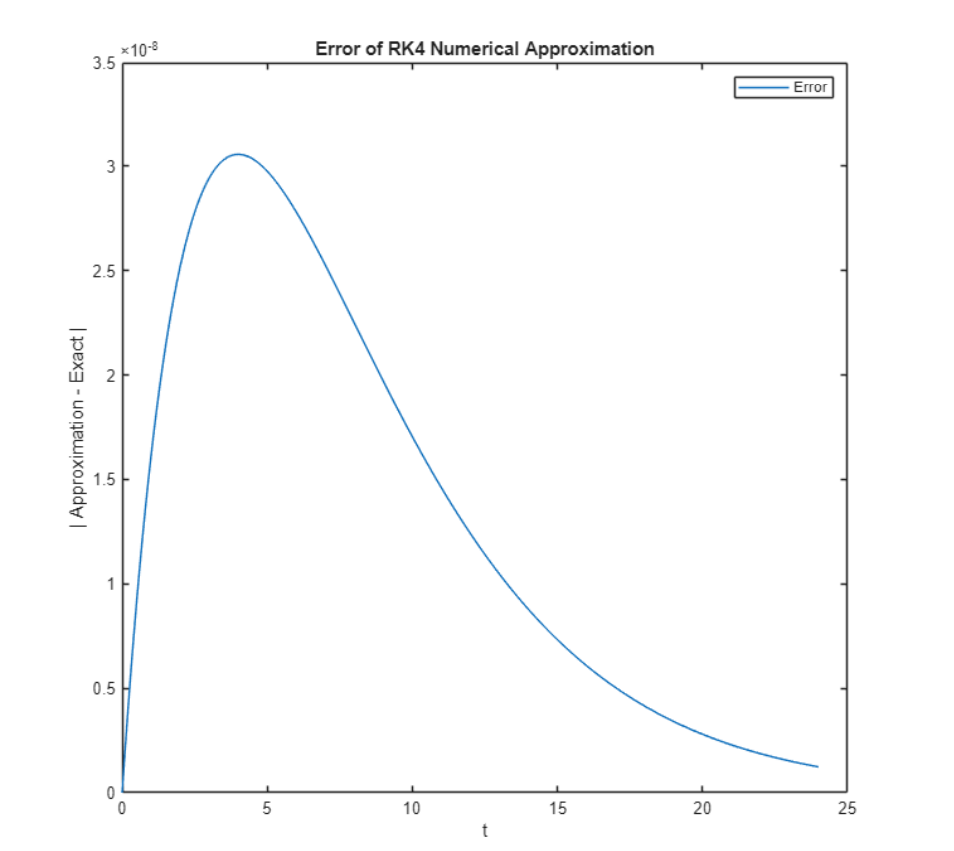
\includegraphics[width=0.5\linewidth]{Screenshot 2025-09-29 181115.png}
    \caption{Runge-Kutta Error}
    \label{fig:placeholder}
\end{figure}

Because the error displayed here peaks at about $3.06\times10^-8$ degrees, we will consider our numerical solution a very good approximation of the actual solution, and use it for calculations going forward. 


\section{Refined models and simulations}
\subsection{Varying outside temperature (Task Set C)}

\subsection{Internal heat sources (Task Set D)}
\subsection{Thermostat control (Task Set E)}

\section{Combined scenarios and safety analysis (Task Set F)}

\clearpage
\section{Results}

\section{Conclusion}

\clearpage
\appendix
\section{Appendix A: Code}
\lstinputlisting{code/tasks.m}


\section{Appendix B: Lengthy Calculations}


\end{document}




